\subsection*{全体概要：この章で学ぶこと}
\addcontentsline{toc}{subsection}{全体概要：この章で学ぶこと}
この章は、ソフトウェアテストを「実行による確認」として扱う。テストは、テスト対象システムを動かし、観測された結果と期待される結果を比べる活動である。ただし、現実のソフトウェアでは、すべての入力、すべての状態、すべての環境を試すことはできない。したがって、テストは常に、限られた資源でどのテストケースを選ぶかという判断を伴う。

\begin{pointbox}{到達目標}
この章を読み終えると、次のことができるようになる。
\begin{itemize}[leftmargin=2em]
  \item 欠陥、障害、テストケース、テストスイート、テストオラクルを区別できる。
  \item 単体テスト、結合テスト、システムテスト、受入テストの違いを説明できる。
  \item 仕様ベース、構造ベース、経験ベース、欠陥ベース、利用ベースのテスト技法を比較できる。
  \item カバレッジ、欠陥密度、信頼性成長モデル、ミューテーションスコアなどの測度の役割を説明できる。
  \item テスト計画、設計、環境構築、実行、インシデント報告、完了判断の流れを説明できる。
  \item 従来型開発、アジャイル、DevOps、TDD、クラウド、AI、ブロックチェーンなどでテストがどう変わるかを説明できる。
\end{itemize}
\end{pointbox}

初学者は、まず「テストは何を証明でき、何を証明できないか」を押さえるとよい。次に、テストのレベル、目的、技法を分けて理解する。最後に、測定、プロセス、ツールの話に進むと、個別技法が実務の中でどう使われるかを理解しやすい。

\begin{figure}[htbp]
\centering
\IfFileExists{assets/generated_figures/ch05/fig-ch05-01.png}{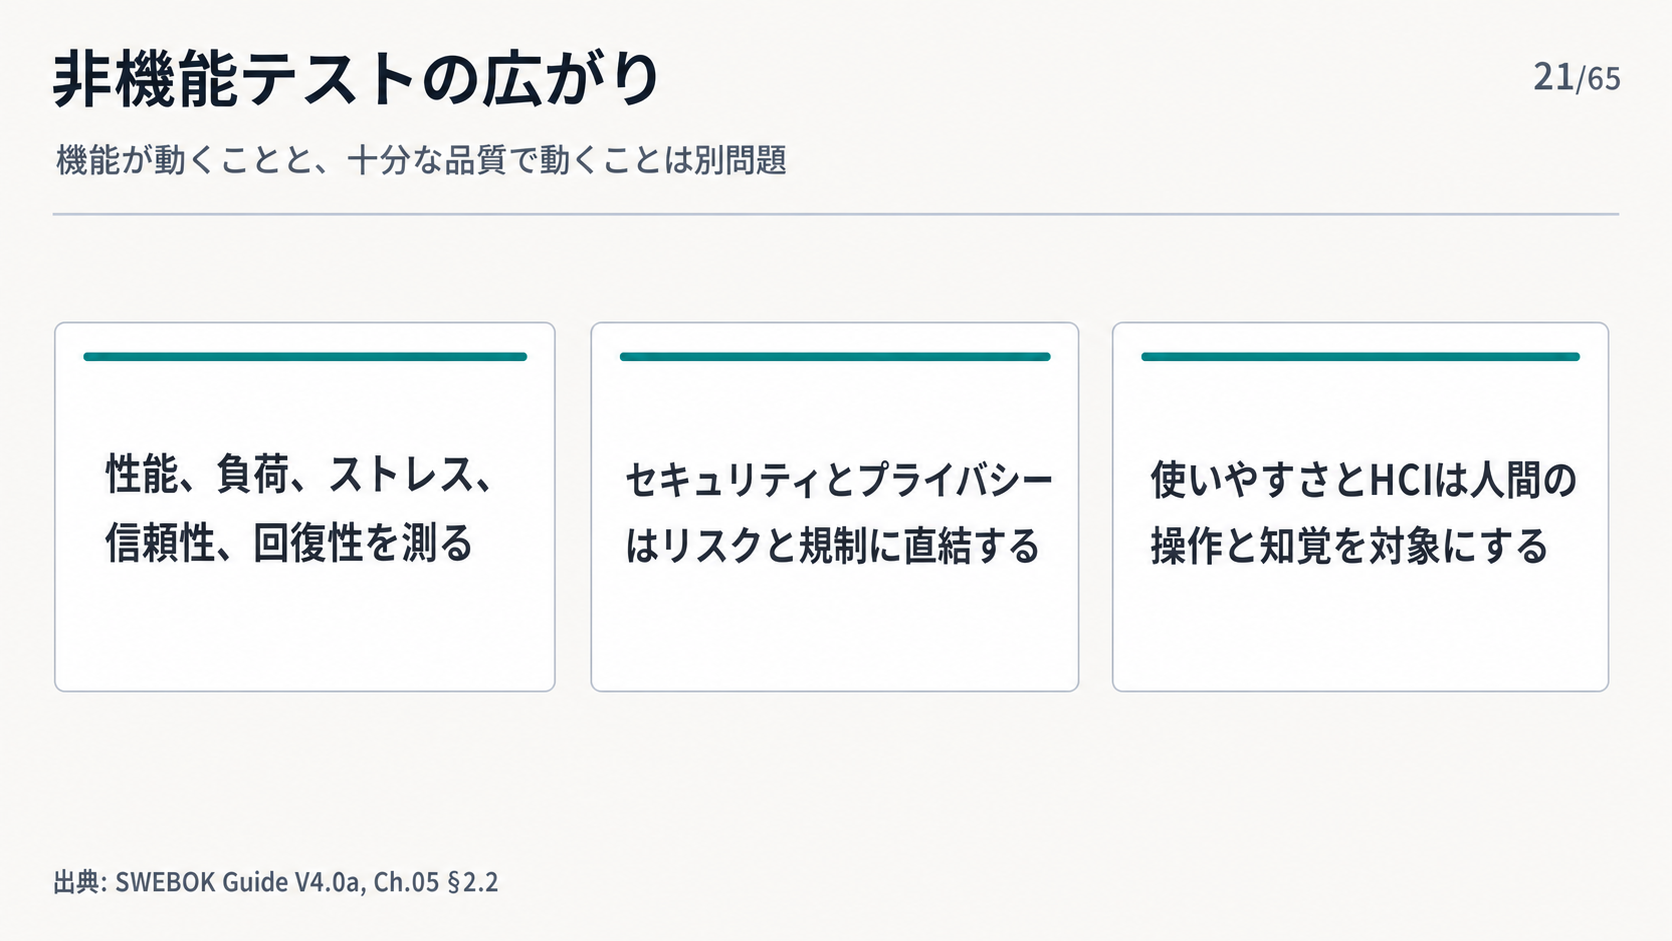
\includegraphics[width=0.96\linewidth]{assets/generated_figures/ch05/fig-ch05-01.png}}{\fbox{\parbox[c][48mm][c]{0.9\linewidth}{\centering 画像生成待ち\\05 章の全体地図}}}
\caption{05 章の全体地図}
\label{fig:ch05-01}
\end{figure}
